\chapter{Revisão Bibliográfica}
\label{cap-revisao-bibliografica}
%TCC:
Este capítulo conta com uma introdução geral ao tema, apresentando o contexto e o problema que será tratado neste trabalho, bem como trabalhos relacionados e bibliografia de apoio.

A Seção \ref{demanda} discorre sobre a transformação digital nos meios de pagamento, correlacionando com seus riscos, e a necessidade de sistemas que assegurem a integridade dos dados e usuários.

A Seção \ref{mercado} aborda o mercado global de sistemas de Antifraude, levantando suas necessidades e motivações e trazendo um apanhado geral de soluções já existentes. Além disso, traz alguns exemplos de aplicações e empresas que, no papel de cliente, buscam empregar antifraude em suas soluções.

A Seção \ref{classificação} apresenta a tarefa de classificação de texto, que está relacionada ao objetivo deste trabalho, definindo como ela funciona e descrevendo possíveis aplicações. Além disso, especifica dificuldades dessa tarefa quando aplicada ao contexto de responder perguntas sobre atributos de perguntas no Mercado Livre.

A Seção \ref{etapas_classificação} explica as variadas etapas que precisam ser seguidas para que seja implementado um modelo de Aprendizado Profundo, que vão desde as etapas que usam métodos clássicos de pré-processamento de texto na área de Processamento de Linguagem Natural (PLN) até etapas que se valem do atual estado da arte que já se consolidou na literatura, como os modelos Transformadores para classificação de texto.

A Seção \ref{relacionados} faz um levantamento de trabalhos relacionados que também implementam classificação de texto, e que são semelhantes ao proposto neste trabalho, considerando o contexto em que são utilizados ou a língua dos exemplos disponíveis em sua base de dados.

\section{Demanda de Antifraude}
\label{demanda}
Com a popularização dos \textit{smartphones} e o advento da \textit{internet}, bancos tradicionais e chamados bancos digitais (sem existência de agência fisíca) passarm a adotar aplicativos para facilitar a gestão de contas, transferências e pagamentos. Essa mudança de comportamento tem sido vista entre os brasileiros: cada vez mais eles passaram a utilizar os meios digitais para operações bancárias, pagamentos e compras \textit{on-line}. De acordo com Rodrigo Mulinari, diretor da Federação Brasileira de Bancos (FEBRABAN), cerca de 70\% das operações bancárias foram feitas via celular, no período de 2019 a 2023, e, neste mesmo período, houve um aumento de 251\% deste uso \cite{febraban2024}.

Um fator que contribuiu para o aumento destes números foi a implementação do Pix, no final do ano de 2020, um método de pagamentos instantâneo que pode ser utilizado em todo o país \cite{febraban2024}.

No entando, o crescimento de transações financeiras \textit{online} tem atraído a atenção de golpistas e indivíduos mal-intencionados, que empregam diversas estratégias para ludibirar vítimas e apropiar-se de seus recursos financeiros ou dados sensíveis. Segundo a pesquisa \cite{datasenado}, golpes digitais atingem cerca de 24\% da população brasileira.

Visando evitar que terceiros utilizem contas bancárias de seus usuários, os bancos adotam ferramentas de Antifraude, que detectam e previnem golpes digitais, assegurando que os dados de seus clientes sejam tratados com segurança e confiabilidade e garantindo que a transação seja legítima do dono da conta.

A segurança em transações online e verificação de identidade requer o uso de diversas ferramentas tecnológicas robustas e eficazes. Dentre elas, destacam-se o Liveness, a Documentoscopia e o FaceMatch, cada qual com funcionalidades específicas e complementares. Liveness é um recurso avançado de biometria facial, e não se limita à simples detecção de um rosto. Ele realiza uma análise multifatorial, considerando aspectos como textura da pele, movimentos faciais sutis, reflexos e até mesmo a detecção de máscaras ou imagens impressas. A verificação vai além da mera presença de um rosto, analisando a dinâmica e características únicas de um rosto real e vivo, rejeitando, assim, tentativas de fraude com fotos, vídeos ou máscaras. Documentoscopia: Essa técnica vai além da simples leitura óptica de caracteres (OCR). A Documentoscopia realiza uma análise forense digital aprofundada do documento, verificando a autenticidade e integridade do documento oficial. Isso inclui a análise de diversos elementos de segurança, como: marcas d'água, microimpressões, elementos holográficos, fios de segurança, padrões de impressão, tipos de papel e tintas utilizadas, além da validação dos dados contra o banco de dados do órgão emissor. Qualquer discrepância ou anomalia é detectada, garantindo a validação da identidade do portador. FaceMatch: Este sistema de comparação biométrica facial utiliza algoritmos avançados para comparar a imagem facial do usuário com um banco de dados, buscando por correspondências. A comparação não se limita à semelhança superficial, mas analisa pontos faciais específicos e características geométricas, garantindo alta precisão e minimizando o risco de falsos positivos. Além disso, a base de dados utilizada é constantemente atualizada e protegida contra acessos não autorizados, garantindo a confiabilidade do processo de verificação.

A combinação dessas tecnologias oferece um sistema de segurança multicamadas, assegurando a verificação de identidade robusta e a prevenção de fraudes em ambientes digitais.

\section{O Mercado de Antifraude}
\label{mercado}
Como apresentado anteriormente, soluções de Antifraude são essenciais se tratando de transações financeiras e segurança bancária. Tais soluções podem ser desenvolvidas em setor próprio da empresa financeira, ou pode ser terceirizada por outras empresas. Dentre as grandes referências de Antifraude, podemos destacar Facetec, iProov, Amazon Rekognition. Abaixo, iremos discorrer melhor sobre suas soluções.

\subsection{FaceTec}
\label{facetec}
A FaceTec é uma empresa estadunidense com sede na California, com foco em implementações tecnológicas de segurança e antifraude. A empresa estabeleceu-se como líder global no segmento de verificação biométrica 3D, oferecendo soluções inovadoras para o mercado de antifraude. Especializada em detecção	 de "liveness" (prova de vida) e correspondência tridimensional, a empresa desenvolveu uma plataforma que combina segurança avançada com experiência do usuário otimizada. Seu sistema patenteado ZoOm-in FaceScan\textsuperscript{\textregistered} cria um FaceMap\textsuperscript{\textregistered} 3D a partir de um vídeo-selfie com duração de 2 a 3 segundos, revolucionando processos de verificação de identidade remota \cite{facetec_2025}.

A tecnologia da FaceTec foi concebida especificamente para combater as crescentes ameaças de fraude digital, posicionando-se como uma barreira eficaz contra roubo de identidade, \textit{phishing} e outros vetores de ataque contemporâneos. Sua abordagem baseada em 3D diferencia-se radicalmente das soluções biométricas tradicionais em 2D, oferecendo níveis de segurança significativamente superiores \cite{facetec_2025}.

O diferencial tecnológico da FaceTec reside em seu sistema de criação de FaceMaps 3D, que captura não apenas características faciais superficiais, mas a estrutura geométrica única do rosto do usuário. Este processo envolve: coleta de mais de 100 quadros de vídeo, analisando a distorção de perspectiva conforme o usuário move o rosto; conversão dos dados 2D em um modelo 3D preciso, utilizando algoritmos de IA e visão computacional; armazenamento seguro nos servidores do cliente, não constituindo um \textit{honeypot} biométrico, pois não contêm os dados de liveness necessários para autenticação \cite{facetec_2025}. 

A empresa estabeleceu um sistema de detecção de \textit{liveness} com novos padrões na indústria, sendo certificado pelos laboratórios NIST/NVLAP (National Institute of Standards and Technology/National Voluntary Laboratory Accreditation Program)\cite{nist_nvlap}. Através de uma abordagem multifatorial, analisa reflexos oculares e textura de pele, profundidade e movimento 3D, características fisiológicas humanas impossíveis de replicar com mídias estáticas. Além disso, a empresa mantém um programa de recompensas por vulnerabilidades (\textit{Spoofy Bounty}) desde 2019, que incentiva a comunidade de segurança a divulgar e reportar fraudes, além de reforçar a confiança em sua capacidade de resistir a tentativas de \textit{spoofing}.

Dentre os vetores de ataques conhecidos, a FaceTec se garante em neutralizar efetivamente os seguintes métodos de fraude digital: fotos e vídeos 2D, estáticas ou em movimento; máscaras e réplicas, de papel, cera ou bonecos realistas; \textit{deepfakes} e avatares; injeção de vídeo \cite{facetec_2025}. 

Efetivamente no mercado global e brasileiro, podemos trazer alguns exemplos, como DocCheck, solução da Exato Digital que utiliza o mapeamento 3D  da FaceTec para validação facial e combate a fraudes em operações digitais; e ClearSale, que oferece a tecnologia FaceTec como uma das opções de liveness em sua plataforma de biometria facial para \textit{e-commerce}, bancos e outros setores \cite{exato_digital_doccheck}.

\subsection{iProov}

A iProov também está entre as líderes globais em verificação biométrica de identidade, especializada em soluções antifraude baseadas em tecnologia de \textit{liveness} e autenticação facial. Fundada em 2011 no Reino Unido, a empresa desenvolveu um sistema patenteado que combina biometria facial, iluminação controlada e IA, para assegurar que um indivíduo é "a pessoa certa, uma pessoa real, autenticando-se no momento" \cite{iproov_2025}. Sua atuação abrange setores críticos como serviços financeiros, saúde e viagens.

A empresa utiliza um sistema de verificação facial tridimensional que diferencia seres humanos reais de \textit{deepfakes}, máscaras, fotos estáticas e vídeos pré-gravados. Seu algoritmo de \textit{"Flashmark"} emprega iluminação controlada para detectar reflexos fisiológicos únicos, como textura da pele e movimento ocular. \cite{iproov_2025}

De acordo com dados da própria empresa, novos vetores de ataque tem tido expressivo crescimento, como ataques de câmeras virtuais nativas, \textit{face swap} e síntese de identidades sintéticas via IA generativa. Sendo assim, através de um Sistema de Gerenciamento de Ameaças Ativas (iSOC), a iProov monitora e atualiza continuamente suas defesas. Neste sentido, a empresa elaborou um relatório recente, que alerta para o mercado de "\textit{Crime-as-a-Service}", onde ferramentas de deepfake são comercializadas a criminosos de baixa qualificação, e ataques de injeção de vídeo, que burlam sistemas tradicionais de verificação. \cite{iproov_threat_2025}

Programas de identidade digital governamental,como o UK Digital Identity \& Attributes Trust Framework, utilizam a iProov para verificação remota de documentos (RG, passaporte) com biometria facial, combatendo roubo de identidade e falsificação, e bancos como o UBS (União de Bancos Suíços) adotaram a iProov para textit{onboarding} digital seguro, reduzindo fraudes em abertura de contas e transações de alto valor.

Dentre os destaques e vantagens competitivas da iProov, podemos destacar seu FAR (\textit{False Acceptance Rate}) de 1 em milhão; neutralidade étnica; evitando vieses; e certificações atendendo a padrões internacionais, como: eIDAS, ISO/IEC 30107-3, e FIDO Alliance. \cite{iproov_2025}

\subsection{Amazon Rekognition Face Liveness}

A Amazon Rekognition Face Liveness é uma solução de detecção de vivacidade facial que utiliza Inteligência Artificial e Visão Computacional para combater fraudes em processos de verificação de identidade digital. Desenvolvida pela Amazon Web Services (AWS), a tecnologia é projetada para diferenciar usuários reais de tentativas de \textit{spoofing}.

Bem como as soluções das empresas citadas anteriormente, a solução da Amazon é capaz de detectar vetores de ataques como vídeos pré-gravados, \textit{deepfakes} e máscaras 3D. 

Através de um vídeo-selfie com duração de 2 a 3 segundos, algoritmos de Machine Learning avaliam reflexos faciais, padrões de iluminação e estrutura 3D do rosto. Alguns diferenciais que a solução de \textit{liveness} da Amazon incluem: um score de confiança, onde valores mais altos indicam maior probabilidade de o usuário ser real, podendo haver um ajuste de \textit{threshold} conforme o risco do caso de uso. Outro diferencial é a jornada do usuário, onde luzes coloridas são emitidas na tela, com intuito de observar a reação dos olhos e pele à essas cores. A conformidade com normativas relevantes, como as diretrizes WCAG 2.1 para acessibilidade e o regulamento eIDAS, que atesta um alto nível de segurança, também constitui um diferencial. \cite{aws_ai_cards_2023}

\begin{figure}[htb]
        \centering
        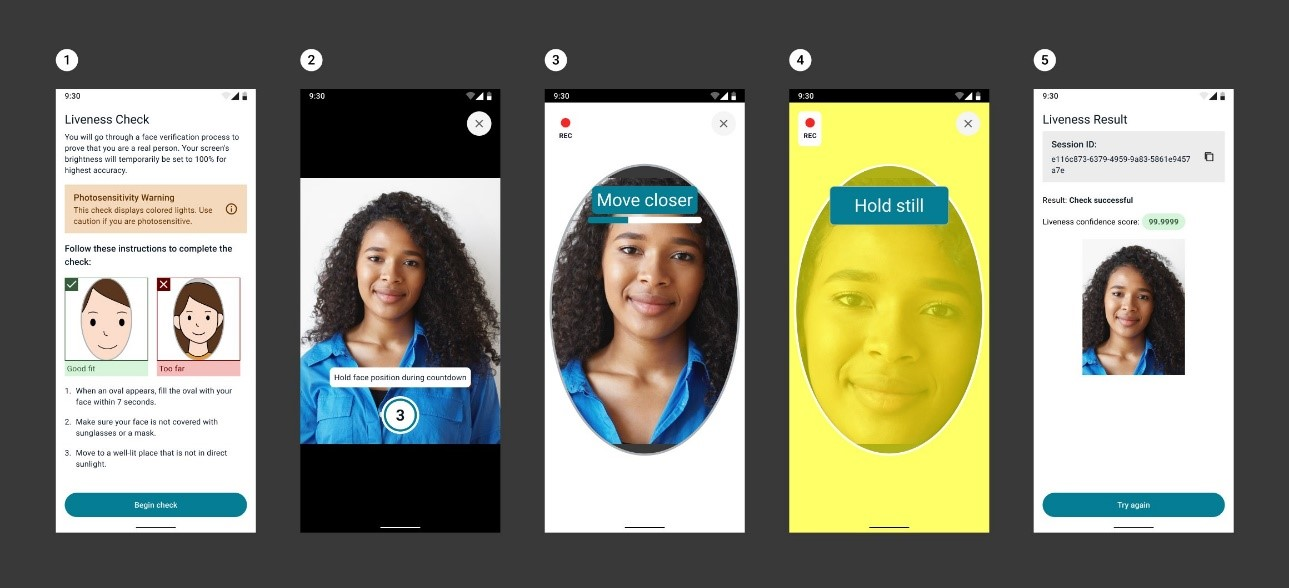
\includegraphics[width=16cm]{figuras/aws_liveness.jpg}
        \caption{Etapas de visualização de tela durante \textit{liveness} desenvolvido pela Amazon.}
        \label{fig:aws_liveness}
\end{figure}

Para assegurar a neutralidade e mitigar vieses discriminatórios, os modelos de ML são treinados com conjuntos de dados (datasets) amplamente diversificados. Essa diversidade abrange variações significativas em tonalidade de pele, faixa etária e identidade de gênero, contribuindo para uma maior equidade na avaliação. \cite{aws_blog_2023}

No mercado de antifraude, a tecnologia encontra diversas aplicações. Em processos de integração digital (\textit{onboarding}), instituições financeiras utilizam a solução para validar a identidade de novos clientes durante a abertura de contas, realizando a comparação biométrica entre a vídeo-selfie e fotografias de documentos oficiais, como carteiras de identidade ou passaportes, frequentemente por meio de interfaces de programação de aplicações (APIs) como a CompareFaces. Adicionalmente, em plataformas de mobilidade urbana, como a Uber, e comércio eletrônico, a tecnologia é implementada para a reautenticação de utilizadores em transações consideradas de alto risco, como transferências bancárias. Setores com restrições etárias, como os de jogos online e tabaco, combinam a detecção de vivacidade com sistemas de estimativa de idade para coibir o acesso de menores. Finalmente, redes sociais e outros serviços digitais empregam esta solução como um substituto avançado para mecanismos de CAPTCHA, exigindo provas de vivacidade para dificultar a proliferação de contas automatizadas (bots) e identidades sintéticas. \cite{aws_rekognition_2023}

\section{Revisão Bibliográfica}
\label{classificação}
O problema a ser estudado neste trabalho, apresentado como classificação de perguntas sobre produtos quanto ao atributo, é definido na literatura como Classificação de Texto (do inglês \textit{Text Classification}). De acordo com a definição apresentada em \cite{survey}, a classificação de texto consiste na seguinte situação: dado um conjunto de instâncias de treino $\mathcal{D} = \{X_1, ..., X_N\}$, onde cada instância $X_i$ é uma sentença textual formada por um conjunto de características (\textit{features}) e está anotada com um valor de classe obtido de um conjunto de k valores discretos indexados como $\{1...k\}$,  treina-se um modelo classificador, que relacionará as características de cada instância de treino a uma das classes. Depois que o treinamento é feito, uma instância de teste, cuja classe é desconhecida, é fornecida ao modelo classificador para que este preveja a classe a qual a instância pertence.

Além de atuar como uma parte integrante de um sistema que responde perguntas de clientes no comércio eletrônico, que é a implementação aqui descrita, a classificação de texto também é muito presente em outros contextos, tais como: obtenção de informações dispostas de forma não estruturada em grandes coleções de documentos \cite{info-retrieval}, filtragem de informações quanto a sua relevância em \textit{streams} de dados \cite{info-filtering}, análise de sentimentos para identificar opinião, sentimento e subjetividade em textos \cite{sentiment-analysis}, sistemas de recomendação que sugerem itens baseados no perfil de interesses do usuário e na descrição do item \cite{recommender-systems}, entre muitos outros \cite{survey2}.

No contexto de resolução de perguntas de clientes reais, a classificação de textos atua para que a pergunta feita seja entendida. Toda pergunta é um questionamento que um cliente possui sobre uma característica de um determinado produto. No contexto deste trabalho, cada classe que o modelo classificador consegue identificar representa uma característica que o produto tem, isto é, representa um atributo do produto. Assim, se um cliente está interessado em saber a marca de uma chave de fenda, ele pergunta "Qual é a marca da chave de fenda?". Esta pergunta, por sua vez, pode ser classificada como uma pergunta sobre o atributo ou classe "marca". Essa forma de responder perguntas encontra diversas dificuldades, que serão discutidas na seção \ref{dificuldades da classificação de perguntas quanto ao atributo}.

\subsection{O Conceito de Atributo no Mercado Livre}
\label{o conceito de atributo no mercado livre}
Os atributos são características dos produtos adicionadas pelos lojistas no formato de pares (nome do atributo, valor do atributo). Eles podem ser acessados por meio de consultas à API do Mercado Livre. Dessa forma, após o modelo classificador prever o nome do atributo ao qual uma pergunta de um cliente real se refere, o valor do atributo pode ser obtido filtrando a resposta da consulta à API e procurando pelo nome do atributo.

Nesse sentido, após a execução da Classificação de Texto pelo modelo classificador, as perguntas feitas na Figura \ref{fig:montagem_perguntas} podem ser respondidas filtrando os nomes de atributos ESIMS\_NUMBER, DISPLAY\_SIZE e MODEL na resposta da consulta à API do Mercado Livre. Os valores dos atributos são 1 (indicando que o celular só possui entrada para um chip), 6,1'' (indicando que o celular possui 6,1 polegadas de tamanho), e iPhone 12 (indicando que o celular é do modelo padrão, e não do modelo Mini), respectivamente. A Figura \ref{fig:resposta_api} mostra a resposta da consulta à API do Mercado Livre.

\begin{figure}
    \begin{subfigure}{\linewidth}
        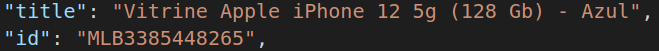
\includegraphics[width=\linewidth]{figuras/api-cabecalho.png}
        \caption{}
        \label{fig:header}
    \end{subfigure}
    
    \begin{subfigure}{0.33\linewidth}
        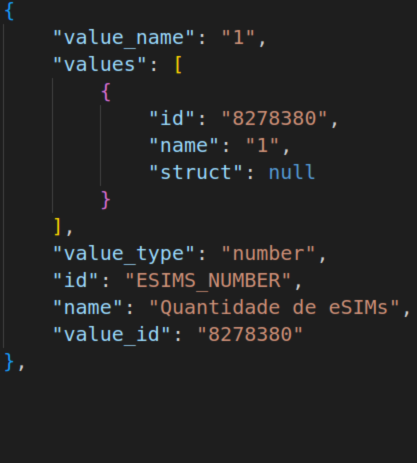
\includegraphics[width=\linewidth]{figuras/api-atributo2.png}
        \caption{}
        \label{fig:display_size}
    \end{subfigure}%
    \begin{subfigure}{0.33\linewidth}
        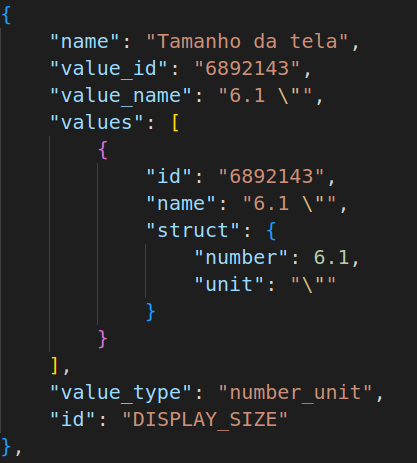
\includegraphics[width=\linewidth]{figuras/api-atributo1.png}
        \caption{}
        \label{fig:esims_number}
    \end{subfigure}%
    \begin{subfigure}{0.33\linewidth}
        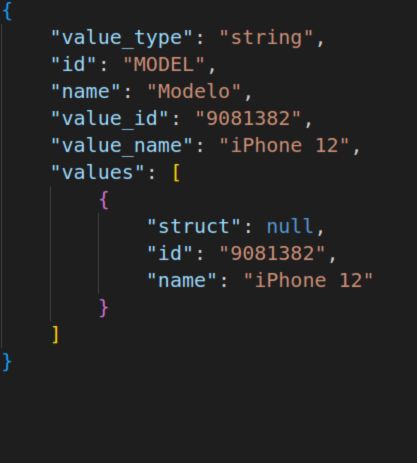
\includegraphics[width=\linewidth]{figuras/api-atributo3.png}
        \caption{}
        \label{fig:model}
    \end{subfigure}

    \caption{Resposta da consulta à API de produtos do Mercado Livre, que retorna nomes e valores dos atributos.
    Em \ref{fig:header}, informações sobre o produto.
    Em \ref{fig:display_size}, a resposta para a pergunta ``Esse iPhone 12 é Dual SIM?''.
    Em \ref{fig:esims_number}, a resposta para a pergunta ``Qual o tamanho desse celular?''.
    Em \ref{fig:model}, a resposta para a pergunta ``Esse é o modelo Mini?''.}
    \label{fig:resposta_api}
\end{figure}


\subsection{Dificuldades da Classificação de Perguntas quanto ao Atributo}
\label{dificuldades da classificação de perguntas quanto ao atributo}
Em Novembro de 2022, o Mercado Livre possuía mais de 7000 atributos únicos, usados para descrever produtos de centenas de subcategorias. Considerando essa condição, estar preparado para responder a perguntas sobre o valor de qualquer atributo, seja ele genérico ou específico, é uma tarefa extremamente difícil, pois ela encontra as limitações citadas a seguir.

\begin{itemize}
    \item Generalização para atributos não vistos nos dados de treino: manter uma base de dados com exemplos de perguntas para cada um dos 7000 atributos é uma tarefa dispendiosa em termos financeiros, e impossível de se realizar manualmente. Além disso, novas categorias de produtos são lançadas todos os dias, o que tornaria esse conjunto de dados obsoleto. Por isso, outros trabalhos da literatura usam estratégias avançadas, como a concatenação de camadas de modelos que não são classificadores \cite{aliexpress}. A técnica proposta no trabalho citado melhorou consideravelmente o reconhecimento de atributos nunca vistos entre os dados de treino, ou seja, aprimorou a habilidade de \textit{zero-shot learning}.
    
    \item Perguntas que se referem à compatibilidade entre produtos: no Mercado Livre existem dois atributos genéricos, o \textbf{COMPATIBLE\_BRANDS} e o \textbf{COMPATIBLE\_MODELS}, que geralmente estão presentes em produtos que são acessórios de objetos maiores, como por exemplo rádios automotivos. É muito comum que as perguntas dessas duas classes diferentes tenham uma estrutura sintática parecida, como exemplificado nas Figuras \ref{fig:ex_model} e \ref{fig:ex_brand}.
    
    \begin{figure}[htb]
        \centering
        \color{blue}- Esse controle é compatível com Xbox Series S?
        \caption{Pergunta que seria classificada como COMPATIBLE\_MODELS.}
        \label{fig:ex_model}
    \end{figure}
    
    \begin{figure}[htb]
        \centering
        \color{blue}- É compatível com micro retífica black\&decker?
        \caption{Pergunta que seria classificada como COMPATIBLE\_BRANDS.}
        \label{fig:ex_brand}
    \end{figure}

    É possível perceber que a classe a que cada exemplo das Figuras \ref{fig:ex_model} e \ref{fig:ex_brand} pertence só pode ser avaliada com base em conhecimento de mundo, que permite distinguir marcas de modelos. Para que um algoritmo de Inteligência Artifical consiga fazer essa distinção com maior assertividade, faz-se necessária uma solução mais específica, como um grande Grafo de Conhecimento com relações entre marcas e modelos de produtos, como explorado em \cite{kg}.
    
    \item Atributos que fazem parte de uma categoria, mas não de outras: cada categoria possui sua lista de atributos válidos. Alguns atributos são mais genéricos e fazem parte da maioria das categorias, enquanto alguns atributos são mais específicos, compõem categorias restritas. Isso faz com que existam atributos análogos entre categorias diferentes. 
    
    Um disco de freio pode ter o atributo \textbf{MATERIAL}, mas uma camiseta só pode ter o atributo \textbf{COMPOSITION}. No entanto, não estamos levando em conta a categoria do produto no momento de fazer a classificação, apenas a pergunta. Isso possibilita que uma pergunta sobre essa camiseta seja classificada como \textbf{MATERIAL}, o que deixaria o cliente sem resposta.
    \item Saudações: os clientes frequentemente introduzem palavras extras, como saudações, para estabelecer a cordialidade entre eles e os atendentes. Isso provoca um ruído desnecessário que pode afetar o resultado final, uma vez que esses cumprimentos também serão fornecidos ao modelo classificador se não forem apropriadamente filtrados.
    \item Variações na ortografia: os clientes possuem diferentes níveis de escolaridade e as perguntas são feitas em um contexto virtual, favorável a abreviações. Esses dois fatores permitem com que uma palavra possa ser escrita das mais variadas formas, o que representa um desafio para os \textit{tokenizadores}, descritos na Seção \ref{pré-processamento dos dados}.
    
    \end{itemize}

\section{Etapas da Classificação de Perguntas Quanto ao Atributo}
\label{etapas_classificação}
A construção de um modelo de classificação de perguntas quanto ao atributo, que pode ser formalizada como uma tarefa de classificação de texto, exige a realização de diversas etapas, que serão descritas nas subseções a seguir.

\subsection{Definição das Classes}
Não é possível, de forma manual, criar uma base de dados com instâncias de todos os atributos existentes para se classificar um produto em um dado \textit{marketplace}. Isso acontece porque aos produtos anunciados nos \textit{marketplaces} podem ser atribuídas centenas ou até mesmo milhares de atributos diferentes. Apesar de existirem modelos pré-treinados que conseguem identificar atributos não usados no treinamento, como em \cite{aliexpress}, torna-se importante ter uma base de dados construída em um conjunto conhecido de classes a fim de avaliar um modelo.

A API de Categorias do Mercado Livre\footnote{\url{https://developers.mercadolivre.com.br/pt_br/categorias-e-atributos}} fornece um recurso \textbf{/attributes} que permite encontrar a lista de todos os atributos de uma dada categoria. Além disso, é possível baixar a árvore de categorias do Mercado Livre\footnote{\url{https://developers.mercadolivre.com.br/pt_br/dump-de-categorias}}, que relaciona todas as categorias e seu grau de parentesco entre si. Um modelo classificador generalista idealmente teria como dados de treino exemplos de perguntas com os atributos que aparecem no maior número de categorias possível, ou seja, os mais genéricos.

\subsection{Coleta de Dados}
\label{coleta de dados}
Os dados provavelmente são a parte mais importante de um sistema de aprendizado de máquina. Em contextos mais simplificados, é facilmente possível obter as bases de dados necessárias para resolver um determinado problema, e elas são constituídos de milhares (ou até mesmo milhões) de instâncias \cite{practical_nlp}. No entanto, na maioria dos projetos de Inteligência Artificial acadêmicos ou comerciais é preciso fazer uso de técnicas de coleta de dados.

Fontes como \cite{practical_nlp} agregaram as técnicas mais empregadas para concluir esta etapa:
\begin{itemize}
    \item Usar uma base de dados pública: consiste em pesquisar se existem bases de dados públicas disponíveis que sejam similares e compatíveis com o problema em questão. Agregadores como o Google Datasets\footnote{\url{https://datasetsearch.research.google.com/}} e o HuggingFace\footnote{\url{https://huggingface.co/datasets}} compilam muitas das opções disponíveis.
    
    \item \textit{Data Scraping}: consiste em encontrar uma fonte de dados relevante na Internet e fazer uso de técnicas de \textit{Web Scraping}, ou seja, obter esses dados de forma que não seja por meio de um programa interagindo com uma API (nem por interação humana). Geralmente esse objetivo é atingido escrevendo um programa que se comunica com um servidor Web, faz uma requisição de dados (muitas vezes em forma de arquivos HTML) e então formata aqueles dados para extrair a informação necessária \cite{web_scaping}.
    \item \textit{Product Intervention}: é uma técnica muito usada por grandes empresas da tecnologia. Quando essas empresas implementam modelos de Inteligência Artificial em seus produtos, os modelos raramente existem de forma isolada do restante do produto. Assim, a técnica de \textit{Product Intervention} consiste em trabalhar juntamente com o time de produto para obter cada vez mais dados diretamente dos usuários, a partir do momento em que estes autorizam. Esses dados são informações relacionadas aos comportamentos que cada usuário teve ao usar aquele produto. Isso acontece por exemplo quando um usuário acessa um \textit{site} de compartilhamento de vídeos, e obtém recomendações de novos vídeos para assistir através de um algoritmo que analisou vídeos previamente assistidos pelo mesmo usuário.
    \item Aumento de dados: consiste em explorar propriedades linguísticas para criar novos textos que são sintaticamente similares aos textos previamente existentes na base de dados.
\end{itemize}


\subsection{Anotação de Dados}
Todas as técnicas de coleta de dados abordadas na Seção \ref{coleta de dados}, exceto o uso de uma base de dados pública, geralmente levam à compilação de dados não-anotados, ou seja, cada sentença coletada ainda não teve a sua classe correspondente identificada. Como os modelos a serem avaliados neste projeto são modelos de classificação de texto, essa informação se faz necessária para o seu treinamento \cite{survey}.

A anotação de dados (ou identificação de classes) é uma tarefa cansativa, demorada e repetitiva, que frequentemente exige o trabalho de uma equipe de anotadores. Além disso, nem sempre é possível saber de forma previsível quantos exemplos anotados serão necessários, uma vez que modelos linguísticos eficazes podem ser construídos com base em uma quantidade de exemplos modesta, desde que os dados de treinamento coincidam com a aplicação desejada \cite{effects_of_corpus_size}.

Depois que as classes estejam manualmente identificadas, uma prática comum na área de Ciência de Dados é dividir os exemplos em dois conjuntos: o de Treino e o de Teste. O conjunto de Treino é composto por aqueles exemplos que serão consumidos durante as iterações de treinamento, enquanto o conjunto de Teste é composto por outros exemplos mantidos fora do treinamento, que não influenciarão as propriedades do modelo e servirão para estimar o quão efetivo um modelo é por meio da comparação da previsão com o valor conhecido \cite{data_science_handbook}. Uma intuição inicial habitualmente tida pelos cientistas é separar 80\% dos exemplos para Treino e 20\% dos exemplos para Teste, seguindo o Princípio de Pareto \cite{80_20}.

Frequentemente não é possível saber quais dados seriam mais adequados para Treino e quais dados seriam mais adequados para Teste. Para resolver esse problema, pode ser usada a técnica de Validação Cruzada. Essa técnica consiste em fazer uma sequência de treinamentos em que cada subconjunto dos dados é usado tanto como conjunto de Treino quanto como conjunto de Teste. Os subconjuntos devem possuir a mesma quantidade de instâncias, e a quantidade de iterações é definida pela quantidade de subconjuntos. Ao final, pode se combinar as métricas dos modelos treinados em cada iteração da sequência (por exemplo, tomando a média) para obter uma melhor métrica da performance do modelo global \cite{data_science_handbook}. 

\subsection{Pré-processamento dos Dados}
\label{pre-processamento dos dados}
Os \textit{softwares} de NLP tipicamente analisam texto dividindo-o em palavras (\textit{tokens}) e sentenças \cite{practical_nlp}. Por isso uma subetapa importante do pré-processamento de dados diz respeito a essas divisões. 

Após as divisões, outros passos são frequentemente efetuados por cientistas de dados, a depender da tarefa específica a qual o modelo treinado se dedicará, assim como do domínio do problema. Esses passos são importantes pelo fato de que um grande dicionário dificulta a tarefa de mineração de dados, por exemplo, no caso de redes neurais. Como redes neurais podem ser caras de se treinar, é importante não desperdiçar capacidade computacional \cite{transformers_book}. Alguns passos comuns a esta etapa são:
\label{pré-processamento dos dados}
\begin{itemize}
    \item \textit{Lowercasing}: consiste em converter todas as letras maiúsculas em minúsculas, deixando o texto todo em caixa baixa \cite{practical_nlp}.
    \item Remoção de \textit{stopwords}: consiste em remover todas aquelas palavras que aparecem com grande frequência no decorrer da base de dados, mas que não contribuem para a semântica da sentença, pois não fornecem nenhuma informação adicional. Ao removê-las, é possível focar nas palavras mais importantes. Alguns exemplos são os artigos, determinantes e pronomes, como ``o'', ``a'', ``os'', ``de'', etc. \cite{practical_nlp} \cite{etaiwi2017impact}.
    \item Remoção da pontuação e/ou números: a remoção de todo tipo de pontuação, tais como pontos de interrogação, vírgulas, pontos finais, entre outros, afeta o resultado de qualquer abordagem de processamento de texto, especialmente aquelas que dependem da frequência de ocorrência de palavras e frases \cite{etaiwi2017impact}.
    \item \textit{Stemming}: é o processo de remover sufixos para reduzir uma palavra de forma que todas as variantes daquela palavra podem se representadas da mesma forma (por exemplo, ``carros'' e ``carro'' são ambos reduzidos para ``carro''). Isso é feito seguindo uma série de regras. Algoritmos de \textit{Stemming} são específicos para cada língua e diferem em termos de performance e acurácia \cite{practical_nlp} \cite{etaiwi2017impact}.
    \item \textit{Lemmatization}: possui algumas similaridades com o \textit{Stemming}, porém consiste em mapear todas as diferentes formas de uma palavra para a sua palavra base. Por exemplo, o adjetivo ``melhor'' se torna ``bom''. Esse processo requer um conhecimento linguístico maior do que o anterior \cite{practical_nlp}.
\end{itemize}


\subsection{Transformação dos Dados}
Para que algoritmos de aprendizado de máquina trabalhem com dados textuais, esses dados devem ser convertidos para uma representação numérica. Se textos são representados como vetores de números, a representação numérica é chamada de \textit{Vector Space Model} (VSM). Diversas abordagens algébricas podem ser feitas para se obter um VSM \cite{practical_nlp}. Elas serão elaboradas nas Seções \ref{bag of words e tf-idf} e \ref{tokenizadores}.

\subsubsection{Bag of Words e TF-IDF}
\label{bag of words e tf-idf}
Duas abordagens clássicas de representação de dados textuais são a \textit{Bag of Words} e a TF-IDF. Essas abordagens são antigas e de relativa fácil implementação, o que faz com que sejam frequentemente consideradas como linhas de base em artigos científicos. Uma referência inicial a \textit{Bag of Words} em um contexto linguístico está em \cite{bag-of-wordsPaper}, onde o autor argumenta que ``língua não é simplesmente uma \textit{bag of words}, mas sim uma ferramenta com propriedades particulares que foram forjadas durante seu uso''. Já a definição da abordagem TF-IDF está em \cite{tf-idfPaper}, onde a autora argumenta que ``termos devem ser ponderados de acordo com a frequência em que aparecem no conjunto''. Logo, em um contexto onde é feita uma pesquisa usando palavras-chave para encontrar documentos relacionados, a correspondência com termos mais específicos é de maior valor do que a correspondência com termos mais frequentes.

A representação de instâncias usando a abordagem \textit{Bag of Words} pode utilizar o formato de uma tabela atributo-valor, onde cada documento $d_i$ é um exemplo da tabela e cada termo (palavra) $t_j$ é um elemento do conjunto de atributos \cite{bag_of_words}.

\begin{center}
\begin{table}[ht]
\caption{Representação de documentos}
\label{table:representação de documentos}
\centering
    \begin{tabular}{|c | c | c | c | c || c|} 
     \hline
      & $t_1$ & $t_2$ & ... & $t_M$ & $C$ \\ [0.5ex] 
     \hline
     $d_1$ & $a_{11}$ & $a_{12}$ & ... & $a_{1M}$ & $c_1$ \\ 
     \hline
     $d_2$ & $a_{21}$ & $a_{22}$ & ... & $a_{2M}$ & $c_2$ \\
     \hline
     ... & ... & ... & ... & ... & ... \\
     \hline
     $d_N$ & $a_{N1}$ & $a_{N2}$ & ... & $a_{NM}$ & $c_N$ \\
     \hline
    \end{tabular}
\end{table}
\end{center}

Cada documento $d_i$ da Tabela \ref{table:representação de documentos} é um vetor $d_i = (a_{i1}, a_{i2}, ..., a_{iM})$, no qual o valor $a_{ij}$ refere-se ao valor associado ao j-ésimo termo do documento $i$. Esse valor pode ser calculado usando diferentes medidas. Se usarmos a medida \textit{tf}, por exemplo, o valor de $a_{ij}$ será a frequência que o termo $t_j$ aparece no documento $d_i$. No entanto, quando algumas palavras aparecem na maioria dos documentos, eles podem não fornecer informações úteis \cite{bag_of_words}.

A TF-IDF (\textit{term frequency–inverse document frequency}) é outra abordagem de ponderação de termos. Considere $T = \{t_1, ..., t_n\}$ como sendo o conjunto de todos os termos que aparecem em todos os documentos da base de dados. Então, um documento $d_i$ é representado por um vetor de valores reais de $n$ dimensões dado por $x_i = (x_{i1}, ..., x_{in})$ com um componente para cada possível termo do conjunto T \cite{tf-idf}. O peso $x_{ij}$ correspondente ao termo $t_j$ do documento $d_i$ é geralmente um produto de três partes: uma que depende da frequência de $t_j$ em $d_i$, uma que depende da frequência de $t_j$ no conjunto de documentos como um todo, e uma parte de normalização que depende de $d_j$. A fórmula mais comum para a ponderação TF-IDF é definida pela Equação \ref{eq_tfidf}, onde $TF_{ij}$ é a frequência do termo (isto é, o número de ocorrências) de $t_j$ em $d_i$; $IDF_{j}$ é o IDF de $t_j$, definido como o $\log{\frac{N}{DF_j}}$, onde $N$ é o número total de documentos; e $DF_j$ é o número de documentos onde $t_j$ aparece \cite{tf-idf}.

\begin{equation}\label{eq_tfidf}
        x_{ij} = TF_i \cdot IDF_j \cdot (\sum_j(TF_{ij}IDF_{j})^2)^{-1/2}
\end{equation}

\subsubsection{Tokenizadores}
\label{tokenizadores}
Os Tokenizadores são formas de representação de dados textuais mais recentes, que representam o atual estado da arte. Mais uma vez, a cada unidade em que se divide o texto uma representação numérica relacionada é gerada. 

É possível tokenizar em relação a caracteres ou a palavras, mas a forma mais habitual de tokenização empregada pelos cientistas de dados atualmente é a \textit{Subword Tokenization}. Ela combina os melhores aspectos das tokenizações por palavras ou caracteres. Por um lado, é desejável que palavras raras sejam divididas em partes menores, o que permite que o modelo lide com palavras complexas e/ou escritas incorretamente. Por outro lado, é desejável que palavras frequentes sejam mapeadas como entidades únicas para que seja possível manter o comprimento da entrada do modelo em um tamanho controlável \cite{transformers_book}. 

O Tokenizador usado por modelos Transformadores, como os que serão descritos na Seção \ref{modelos ou algoritmos classificadores de texto}, é o WordPiece \cite{wordpiece1} \cite{wordpiece2}, apresentado pelo Google como um dos componentes do seu modelo BERT, aplicado neste trabalho. Ao oferecer como exemplo a sentença ``Tokenizing text is a core task of NLP'' ao \textit{framework} Transformers \cite{hf_transformers_paper}, que implementa o WordPiece, é feita a tokenização. Na prática, trechos de palavras são mapeados a números inteiros. A Figura \ref{fig:input_ids} mostra esse mapeamento.

\begin{figure}[htb]
        \centering
        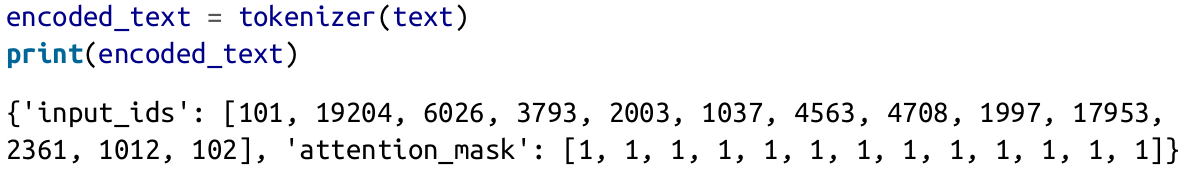
\includegraphics[width=14cm]{figuras/input_ids.png}
        \caption{Mapeamento de \textit{subtokens} a números inteiros únicos. Fonte: \cite{transformers_book}}
        \label{fig:input_ids}
\end{figure}

Ao converter os números inteiros para tokens, como mostrado na Figura \ref{fig:tokens}, é possível entender como as palavras são divididas. Dois tokens especiais, o [CLS] e o [SEP], foram adicionados ao início e ao fim da sentença. Além disso, as palavras passaram por \textit{lowercasing}, subetapa de pré-processamento explicada em \ref{pre-processamento dos dados}. Outro detalhe que se pode observar é que ``tokenizing'' e ``NLP'' foram divididas em dois tokens. Isso faz sentido, uma vez que uma das premissas desse tokenizador é dividir palavras raras em unidades menores \cite{transformers_book}.

\begin{figure}[htb]
        \centering
        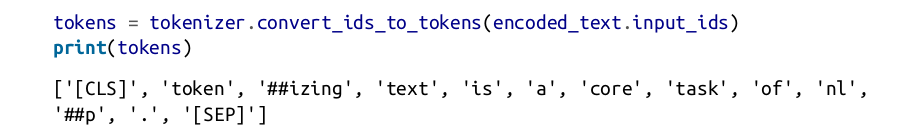
\includegraphics[width=14cm]{figuras/tokens.png}
        \caption{Resultado da conversão de números inteiros únicos para tokens. Fonte: \cite{transformers_book}}
        \label{fig:tokens}
\end{figure}

\subsection{Algoritmos Classificadores de Texto}
\label{modelos ou algoritmos classificadores de texto}
A tarefa de classificação de textos é estudada desde muito tempo, e portanto, diversos métodos de cumpri-la foram implementados ao longo dos anos. \citeonline{survey} e \citeonline{survey2} compilaram em suas pesquisas diversas técnicas de aprendizado de máquina para classificação de texto, tais como: algoritmo de Rocchio \cite{rocchio}; \textit{boosting} \cite{boosting} e \textit{bagging} \cite{bagging}, que são algoritmos de votação; regressão logística \cite{logistic_regression}; Naïve Bayes \cite{naive_bayes}; \textit{k-nearest neighbor} \cite{k_nearest}; \textit{support vector machines} (SVMs) \cite{svm}; árvores de decisão \cite{decision_tree} e \textit{random forests} \cite{random_forests}; algoritmos baseados em redes neurais; dentre muitos outros.

No entanto, este trabalho se dedica a explorar algumas das técnicas mais recentes de classificação de texto, especificamente as que são baseadas em \textit{Deep Learning}. \citeonline{survey3} compilaram em sua pesquisa diversas dessas técnicas, tais como: \textit{transformers} \cite{attention_is_all_you_need} ou \textit{pre-trained language models}; \textit{feed-forward networks}, como por exemplo o modelo DAN \cite{dan}; modelos baseados em RNNs, como o MT-LSTM \cite{mt-lstm}; modelos baseados em CNNs, como o modelo DCNN \cite{dcnn}; \textit{memory-augmented networks}, como a NSE \cite{nse}; dentre muitos outros. Dentre elas, duas arquiteturas diferentes de Transformadores foram escolhidas para esse projeto, BERT e DIETClassifier.

\subsubsection{BERT}
\label{bert_subsubsection}
O BERT é um modelo de Transformador \cite{attention_is_all_you_need}, e foi apresentado em \cite{bert}. Transformadores são algoritmos de \textit{Deep Learning} que possuem como diferencial os mecanismos de auto-atenção, cujo desenvolvimento é explicado em ordem cronológica nos parágrafos seguintes.

Há alguns anos, era comum que tarefas como a tradução fossem resolvidas usando a arquitetura \textit{encoder}-\textit{decoder}. Isto é, uma frase qualquer em Inglês era convertida para uma representação vetorial, chamada de \textit{last hidden state}, dentro de uma arquitetura chamada de \textit{encoder}, composta de redes neurais recorrentes (RNNs). Na outra ponta, essa representação vetorial era convertida de volta para uma outra língua, como o Alemão, na arquitetura conhecida como \textit{decoder}, feita também de RNNs. Porém, essa solução trazia um problema: a representação vetorial tinha dimensões fixas, o que fazia com que informações fossem perdidas em longas sentenças \cite{transformers_book}. Essa solução era aplicada antes do advento dos mecanismos de atenção.

Os mecanismos de atenção vieram como uma solução para esse problema de perda de informação. A Figura \ref{fig:decoder_attention} retrata como funciona uma iteração desses mecanismos. Com eles, ao invés de produzir uma única representação vetorial para a frase em Inglês, o \textit{encoder} produz uma representação vetorial diferente para cada palavra da frase. Ao final do Passo 1, todas as representações vetoriais são enviadas para o \textit{decoder}. Após receber as representações, o \textit{decoder} fornece para cada uma delas uma pontuação no Passo 2. Essa pontuação, que é um número inteiro simples, é fornecida como entrada para a função softmax(), que por sua vez é uma função que transforma um vetor de números em uma distribuição de probabilidades, onde o maior elemento do vetor recebe um grande peso (observe a probabilidade associada a cada elemento no Passo 3 da Figura \ref{fig:decoder_attention}). A função softmax() é descrita pela Equação da Figura \ref{eq_softmax}. Finalmente, no Passo 4, cada representação vetorial é multiplicada pelo seu valor de softmax(), o que faz com que representações vetoriais que tinham grandes pontuações no Passo 2 sejam amplificadas, em detrimento das representações vetoriais que tinham baixas pontuações \cite{attention_explained} \cite{attention_paper1} \cite{attention_paper2}.

\begin{figure}[h!t]
  \centering 
    $\text{softmax}(x_i) = \dfrac{\exp(x_i)}{\sum_j \exp(x_j)}$
    \caption{A softmax() de um elemento de um vetor é a exponencial desse elemento de vetor dividida pela soma das exponenciais de todos os elementos do vetor.}
    \label{eq_softmax}
\end{figure}    

\begin{figure}[htb]
        \centering
        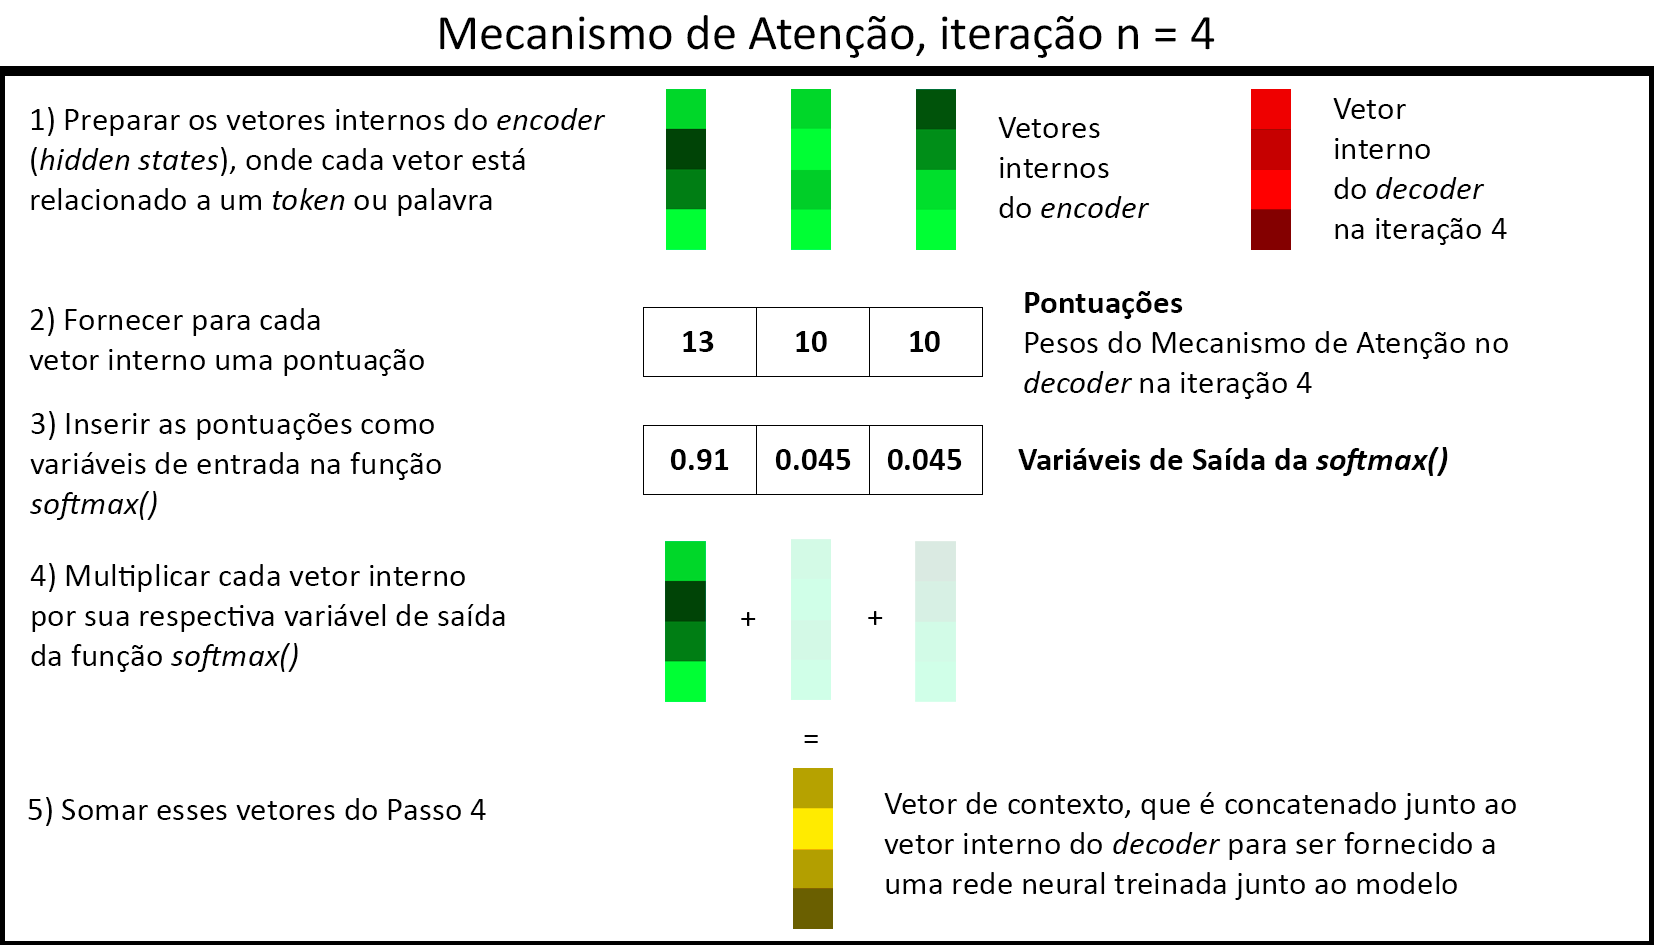
\includegraphics[width=14cm]{figuras/mecanismo_de_atencao.png}
        \caption{Mecanismo de atenção em um \textit{decoder}. Fonte: \cite{attention_explained}}
        \label{fig:decoder_attention}
    \end{figure}

Os mecanismos de Auto-atenção são uma evolução dos mecanismos de Atenção, e foram apresentados como uma característica dos Transformadores. A principal ideia por trás deles é que, ao invés de usar uma representação vetorial fixa para cada \textit{token}, eles usam a sequência inteira para calcular uma média ponderada de cada representação vetorial \cite{transformers_book}. Dessa forma, quando uma sentença possui a palavra ``manga'', por exemplo, é possível diferenciar pelo contexto se a sentença se refere à fruta ou à parte da camisa, e assim produzir uma representação vetorial que leva em consideração esse significado.

A Tabela \ref{tab:attentions} compila os principais pontos dos mecanismos referenciados nos três parágrafos anteriores: pré-atenção (o que era aplicado antes do avento dos mecanismos de atenção), Atenção, e Auto-atenção. Ela considera uma tarefa de tradução de sentenças, onde o Codificador (\textit{encoder}) recebeu uma sentença em Inglês, por exemplo, e o Decodificador (\textit{decoder}) deve fornecer como saída a tradução da sentença em Português. 

\begin{table}[htb]
\centering
\caption{Os três mecanismos: pré-atenção, Atenção e Auto-atenção}
\begin{tabular}{|p{5cm}|p{10cm}|}
\hline
Mecanismo & Principais Pontos \\
\hline
Pré-atenção & O Decodificador tem acesso a apenas um dos vetores (hidden states) gerados pelo Codificador, e esse vetor possui tamanho fixo. Isso faz com que tanto frases simples quanto textos longos sejam representados por um vetor de mesmo tamanho, o que faz muitas informações serem perdidas quando usando textos longos. \\
\hline
Atenção (Attention) & O Decodificador tem acesso a todos os vetores (hidden states) gerados pelo Codificador. Esses vetores são gerados sequencialmente, ou seja, um a cada palavra. Isso significa que na iteração 3, por exemplo, existem três vetores. O Mecanismo de Atenção consiste em fornecer um peso para cada um desses vetores para assim saber quais vetores merecem mais foco, ou mais atenção, a cada iteração. A vantagem é que se torna possível representar adequadamente textos longos, assim como se torna possível criar uma associação entre as palavras ``casa'' e ``house'', por exemplo, mesmo que ``casa'' seja a primeira palavra da frase em Português e ``house'' seja a última palavra da frase em Inglês. \\
\hline
Auto-atenção/Transformadores (Self-attention/Transformers) & Os pesos dos vetores que definem cada palavra são aprendidos levando em consideração apenas o Codificador. A vantagem é que isso permite obter vetores contextualizados - isto é, obter um vetor diferente para ``manga'', a fruta, do vetor que seria gerado para ``manga'', a parte da camisa. Esse aprendizado é feito ponderando outras palavras do contexto daquela sentença. \\
\hline
\end{tabular}
\label{tab:attentions}
\end{table}

O BERT, sigla para \textit{``Bidirectional Encoder Representations from Transformers''}, se destaca entre os demais Transformadores pelo fato de criar representações vetoriais profundas bidirecionais, isto é, considerando o contexto à esquerda e o contexto à direita de uma determinada palavra \cite{bert}. Para isso, ele usa apenas o \textit{encoder} da arquitetura dos Transformadores, e é pré-treinado em bases de dados extensas: o \textit{BookCorpus} \cite{bookcorpus_paper} e a \textit{Wikipedia}\footnote{\url{https://en.wikipedia.org/}} em inglês. Essas representações foram aprendidas de forma bidirecional automaticamente ao fornecer uma base de dados de Treino composta em 80\% por sentenças com palavras aleatoriamente deixadas em branco (chamadas de palavras mascaradas em \citeonline{bert}), como ilustra a Figura \ref{fig:ex_mlm}. Isso fez com que o modelo se tornasse assertivo em predizer qual palavra melhor completaria o espaço em branco fornecido. No exemplo da Figura \ref{fig:ex_mlm}, ao considerar ``Eu estou'' de um lado e ``sorvete'' do outro, as opções se tornam restritas: se restringem a palavras como ``tomando'', ``comendo'', ``lambendo''. Não seria possível ter tamanha assertividade na resposta se o modelo considerasse apenas ``Eu estou'' e tentasse predizer a palavra restante.

\begin{figure}[htb]
    \centering
    \color{blue}Eu estou tomando sorvete$\rightarrow$ Eu estou \_\_\_\_ sorvete
    \caption{Como os criadores do modelo BERT tinham a intenção de que ele aprendesse a considerar tanto palavras que estão ao início de uma sentença quanto palavras que estão ao final de uma sentença, para que assim as representações vetoriais das palavras levassem em conta o contexto, 80\% da base de dados de Treino era composta de sentenças com palavras mascaradas, isto é, em branco.}
    \label{fig:ex_mlm}
\end{figure}

Um fator que tornou o BERT muito popular foi a praticidade de sofrer \textit{fine-tuning}, isto é, de receber uma camada de saída a mais e ter a possibilidade de ajustar apenas os pesos dela: isso tornou o modelo eficiente em muitas outras tarefas específicas, como classificação de texto. O BERT ajudou a definir o estado da arte, e por isso foi precursor de vários modelos frequentemente usados nos dias atuais, como os modelos RoBERTa \cite{roberta_paper} \cite{transformers_book}.

\subsubsection{DIETClassifier}
O DIETClassifier \cite{diet_classifier} também é um modelo de Transformador \cite{attention_is_all_you_need}. Sua característica mais marcante é o fato dele possibilitar que duas tarefas sejam executadas ao mesmo tempo sobre uma entrada de texto: ele faz classificação de intenções e reconhecimento de entidades na mesma iteração, normalmente associadas a uma interface de conversação usuário-máquina, como mostra a Figura \ref{fig:diet_schema}. Enquanto a classificação de intenções se assemelha muito à tarefa de classificação de texto abordada aqui, e está relacionada a entender qual objetivo o usuário tinha ao enviar uma determinada frase, o reconhecimento de entidades busca categorizar palavras específicas da sentença em classes previamente vistas pelo modelo \cite{diet_blog}.

\begin{figure}[htb]
        \centering
        \includegraphics[width=14cm]{figuras/tarefas_do_DIET.png}
        \caption{As duas tarefas que são executadas ao mesmo tempo por um classificador DIET: classificação de intenções e reconhecimento de entidades.}
        \label{fig:diet_schema}
\end{figure}

Outros pontos importantes levantados pelos autores do DIETClassifier são a sua arquitetura modular e seus bons resultados comparados a modelos pré-treinados, como o BERT. A modularização se dá porque é possível usar as representações vetoriais aprendidas por modelos como o próprio BERT como uma de suas camadas, e mesmo assim montar uma arquitetura completa que tenha o classificador DIET como camada de saída. Os bons resultados se devem ao fato de que arquiteturas montadas com o DIET podem ter resultados tão bons quanto os demonstrados por modelos maiores, e mesmo assim chegam a ser até 6x mais rápidas de se treinar \cite{diet_classifier} \cite{diet_blog}.

\subsection{Métricas de Desempenho}
\label{métricas_de_desempenho}
As matrizes de confusão são um tipo de visualização que permite entender as nuances do desempenho dos modelos treinados, classe por classe. Nesse tipo de gráfico, as linhas representam as classes verdadeiras, enquanto as colunas representam as classes previstas pelo modelo em questão (a representação em linha ou coluna varia entre trabalhos). 

Suponha que um problema de Processamento de Linguagem Natural foi apresentado, onde um modelo de Inteligência Artificial foi treinado para classificar avaliações dos usuários sobre um determinado filme em \textbf{Bom}, \textbf{Razoável} e \textbf{Ruim}. Esse modelo obteve o resultado retratado na matriz de confusão da Figura \ref{fig:cm_example}. Ao olhar o termo da primeira coluna com a primeira linha, percebe-se que 3 avaliações \textbf{Bom} foram classificadas como \textbf{Bom} pelo modelo treinado. Por outro lado, ao olhar o termo ao lado vê-se que 4 avaliações \textbf{Bom} foram classificadas como \textbf{Razoável} pelo modelo treinado, o que está incorreto.   Dessa forma, um modelo que consegue prever corretamente a opinião dos espectadores em cada avaliação em todas as avaliações de um determinado conjunto teria uma matriz de confusão diagonal (os únicos termos diferentes de zero seriam aqueles da diagonal principal) \cite{metrics_survey}.

\begin{figure}[htb]
        \centering
        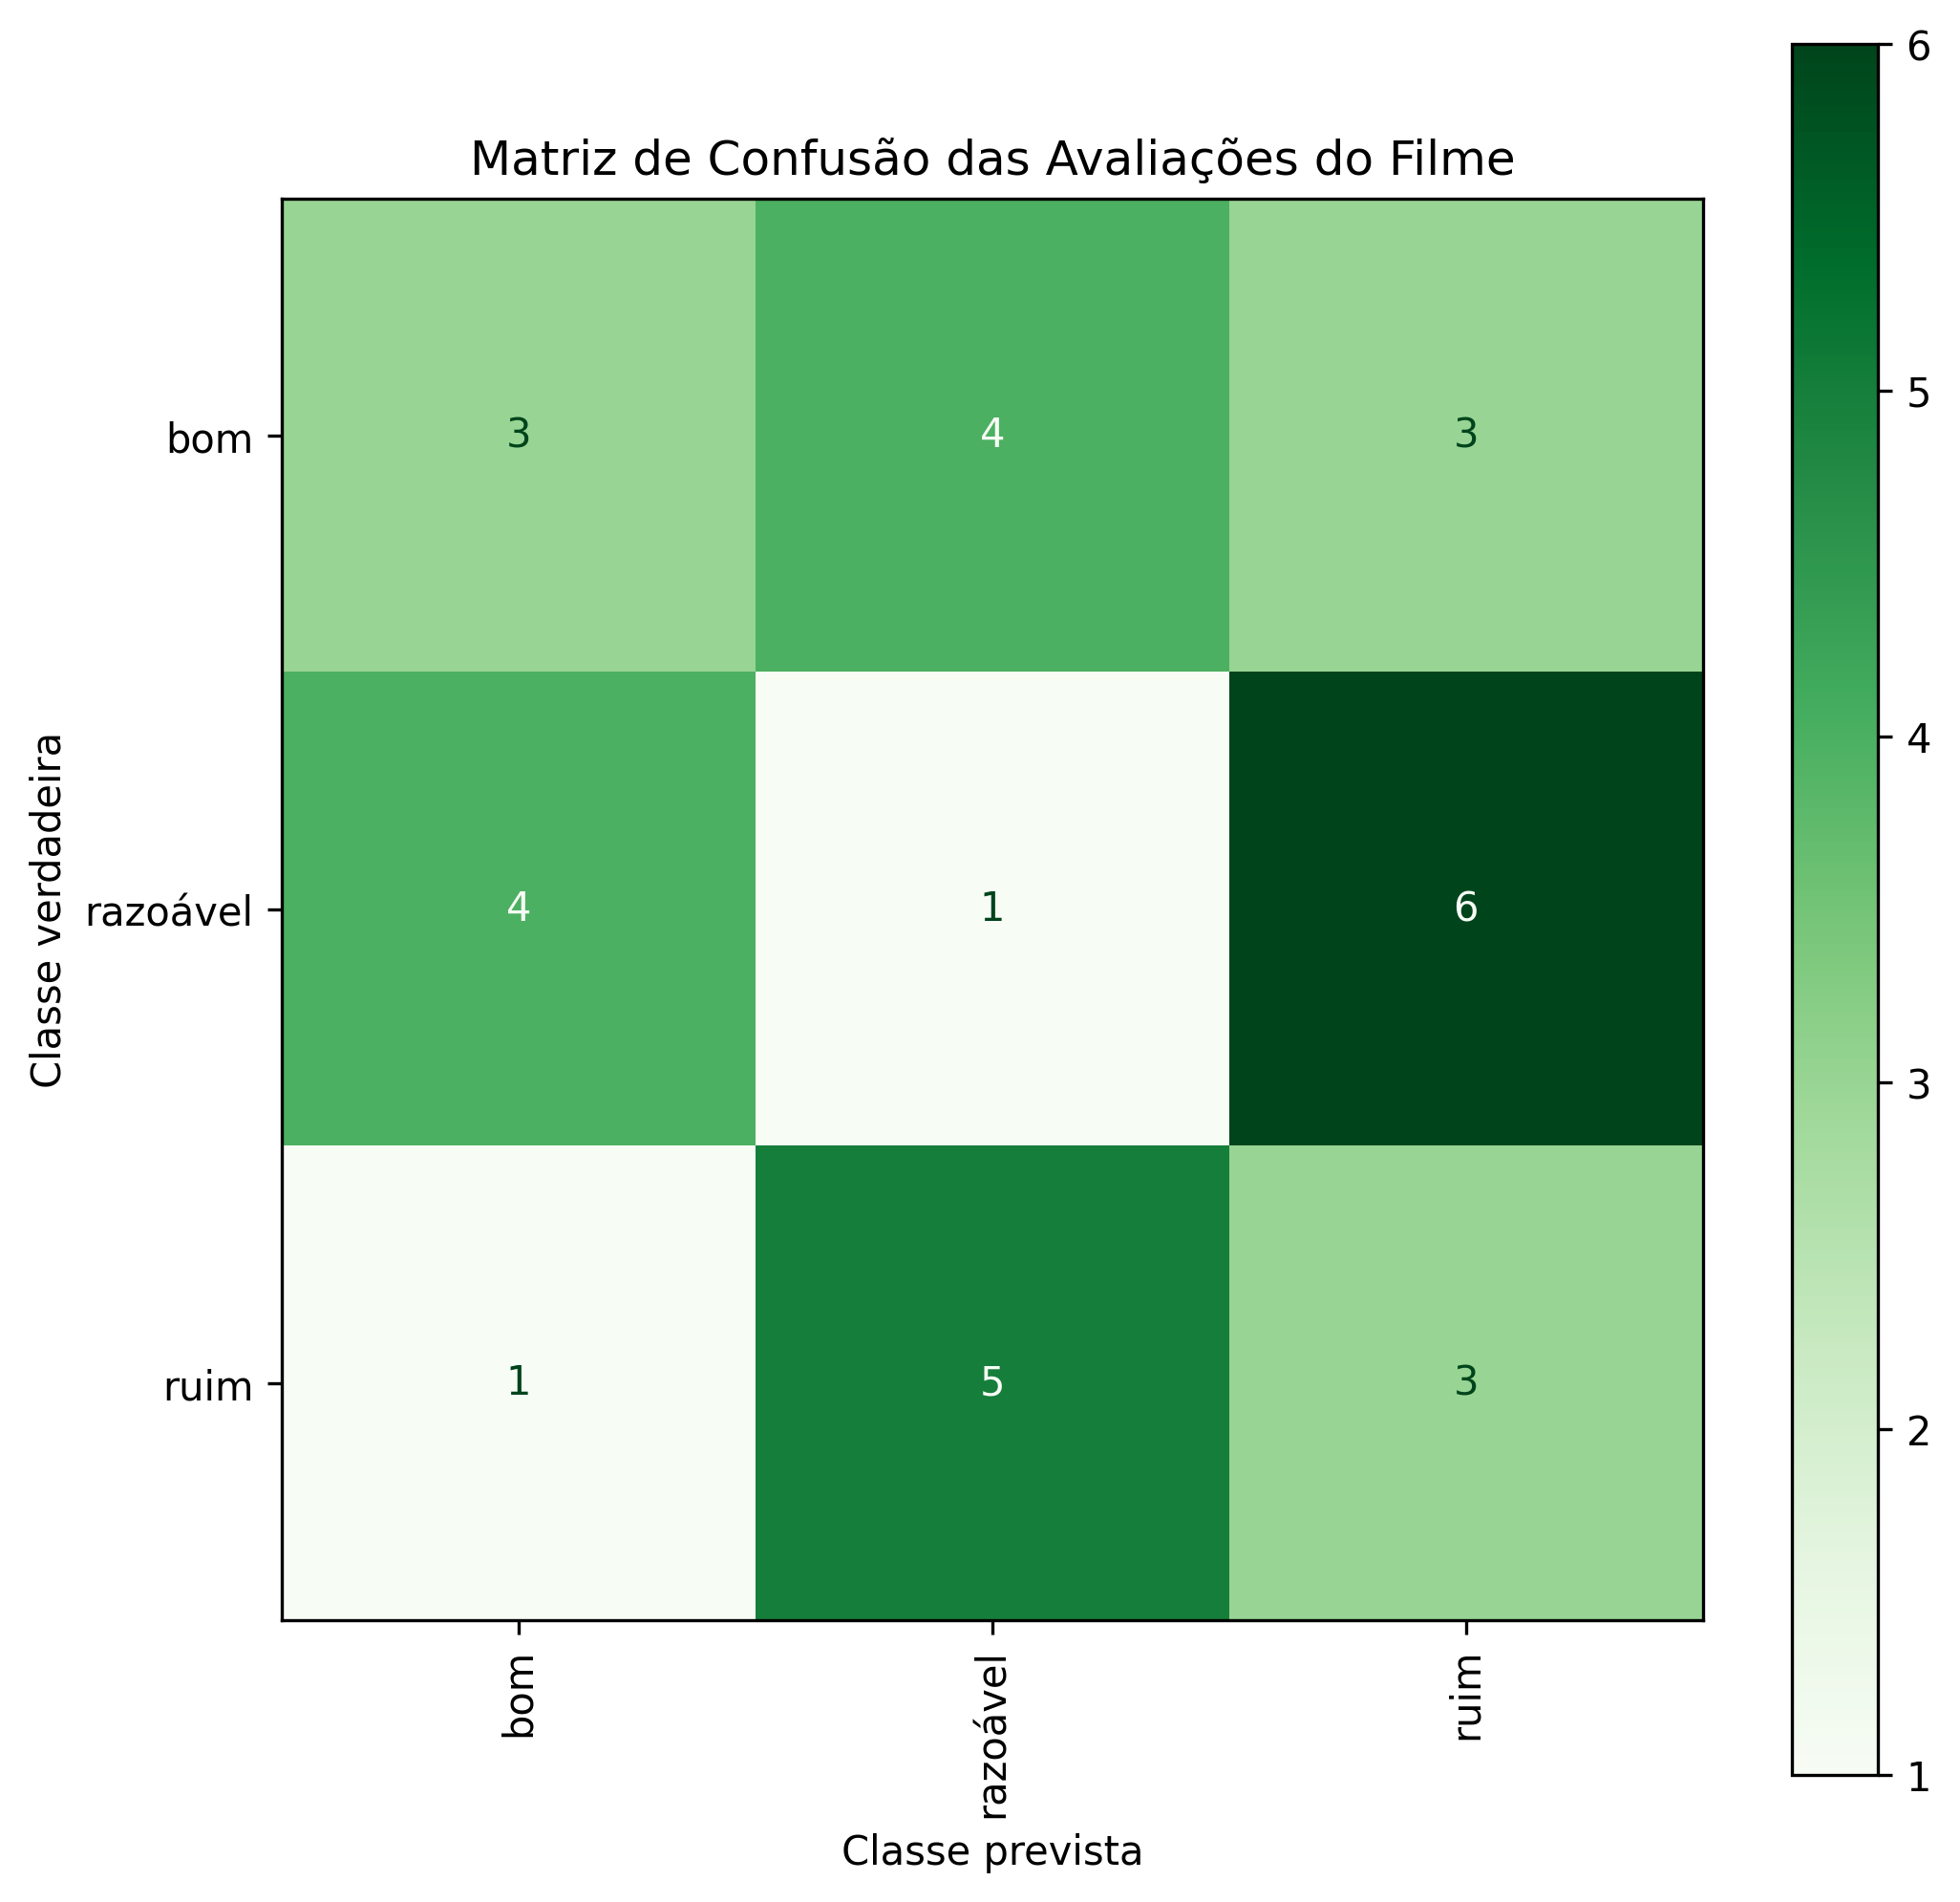
\includegraphics[width=14cm]{figuras/exemplo_filmes.png}
        \caption{Exemplo de visualização de Matriz de Confusão, que será esmiuçado em seções posteriores.}
        \label{fig:cm_example}
\end{figure}

Soluções para problemas de classificação multi-classe, como o abordado neste trabalho, devem ser avaliadas por um conjunto de métricas específico. Trabalhos como a \textit{survey} conduzida em \cite{metrics_survey} se dedicaram a levantar as características dos indicadores de desempenho mais comuns para esse tipo de tarefa, o que é fundamental para a comparação entre os desempenhos dos diferentes modelos treinados. Algumas métricas permitem avaliar a predição de exemplos como um todo. Outras métricas permitem avaliar o quão boa é a predição de uma determinada classe em comparação com outras classes. O engenheiro de aprendizado de máquina deve entender qual tipo de resultado é mais importante e escolher as métricas adequadas se baseando nisso. Entre as métricas mais conhecidas pela literatura, estão:

\begin{itemize}
    \item \textbf{Acurácia}: reflete o quão próximo um dado conjunto de observações (ou previsões, no contexto de Inteligência Artificial) está próximo dos seus valores verdadeiros. Ela considera a soma de todos os elementos classificados corretamente no numerador, enquanto o denominador soma os elementos classificados corretamente com os classificados incorretamente. Assume valores entre 0 e 1 \cite{metrics_survey}.
    \begin{equation}\label{eq_accuracy}
        \text{Acurácia} = \dfrac{TP + TN}{TP + TN + FP + FN}
    \end{equation}
    Na fórmula de Acurácia:
        \begin{itemize}
            \item TP: \textit{true positives}, ou verdadeiros positivos, que é quando um exemplo da classe Positiva é classificado como um elemento da classe Positiva.
            \item TN: \textit{true negatives}, ou verdadeiros negativos, que é quando um exemplo da classe Negativa não é classificado como um elemento da classe Positiva.
            \item FP: \textit{false positives}, ou falsos positivos, que é quando um exemplo da classe Negativa é classificado como um elemento da classe Positiva.
            \item FN: \textit{false negatives}, ou falsos negativos, que é quando um exemplo da classe Positiva é classificado como um elemento da classe Negativa.
        \end{itemize}
    A Acurácia é calculada sobre todo o conjunto avaliado, considerando os exemplos de todas as classes. Existem classes com mais exemplos e classes com menos exemplos. Isso indica que classes mais populadas terão um maior peso em comparação com as classes menos populadas no valor de Acurácia \cite{metrics_survey}.
    \item \textbf{Precisão}: é a proporção de exemplos que o modelo previu como pertencentes à classe Positiva que realmente são daquela classe, ou seja, ela representa o quanto é possível confiar em um modelo quando ele prevê que um exemplo é de uma dada classe. É uma métrica dada para cada uma das classes no contexto de classificação multi-classes. Assume valores entre 0 e 1 \cite{metrics_survey}. A Precisão de uma classe $k$ será igual a (Eq. \ref{eq_precision}):
    \begin{equation}\label{eq_precision}
        \text{Precisão}_k = \dfrac{TP_k}{TP_k + FP_k}
    \end{equation}
    Ao final, caso seja preciso obter uma métrica de Precisão generalizada para todas as classes, pode-se fazer uma média ponderada considerando cada valor encontrado na (Eq. \ref{eq_precision}), o que tira o efeito do desbalanceamento no número de exemplos entre as classes \cite{sk}.
    \item \textbf{Revocação}: considerando todos os exemplos que a classe Positiva possui, indica a porcentagem de quantos foram corretamente identificados como pertencentes a essa classe. É uma métrica dada para cada uma das classes no contexto de classificação multi-classes. Assume valores entre 0 e 1 \cite{metrics_survey}. A Revocação de uma classe $k$ será igual a (Eq. \ref{eq_recall}):
    \begin{equation}\label{eq_recall}
        \text{Revocação}_k = \dfrac{TP_k}{TP_k + FN_k}
    \end{equation}
    Ao final, caso seja preciso obter uma métrica de Revocação generalizada para todas as classes, pode-se fazer uma média ponderada considerando cada valor encontrado na (Eq. \ref{eq_recall}), o que tira o efeito do desbalanceamento no número de exemplos entre as classes \cite{sk}.
    \item \textbf{\textit{F1-Score}}: é uma métrica que agrega as métricas de Precisão e Revocação em uma fórmula de média harmônica. Assim, torna-se possível encontrar a melhor relação entre as duas quantidades. É uma métrica dada para cada uma das classes no contexto de classificação multi-classes. Assume valores entre 0 e 1 \cite{metrics_survey}. O \textit{F1-Score} de uma classe $k$ será igual a (Eq. \ref{eq_f1}):
    \begin{equation}\label{eq_f1}
        {F1}_k = 2\cdot\dfrac{\text{precisão} \cdot \text{revocação}}{\text{precisão} + \text{revocação}}
    \end{equation}
    Ao final, caso seja preciso obter uma métrica de \textit{F1-Score} generalizada para todas as classes, pode-se fazer uma média ponderada considerando cada valor encontrado na (Eq. \ref{eq_f1}), o que tira o efeito do desbalanceamento no número de exemplos entre as classes \cite{sk}.
\end{itemize}

\section{Trabalhos Relacionados}
\label{relacionados}
O estudo da implementação de modelos de aprendizado de máquina para Classificação de Texto é amplo, distribuído entre diferentes tipos de aplicações pelo mundo todo. Alguns dos muitos trabalhos nesse campo se assemelham com o trabalho apresentado por também estarem no contexto do \textit{e-commerce}, enquanto outros são similares porque sua base de dados também é composta por exemplos em Português \cite{survey}. 

Em \cite{relacionado_pt}, o autor usa uma base de dados em Português para classificar perguntas sobre conhecimentos gerais em relação à classe daquela pergunta, como Localidade, Pessoa, etc. Ele então combina essa técnica com reconhecimento de entidades e recuperação da informação para percorrer milhares de documentos e obter a resposta. O pré-processamento é feito a partir de \textit{Lowercasing} e do uso dos algoritmos TF-IDF e \textit{Word2Vec} \cite{word2vec} individualmente ou em conjunto (chamado pelo autor de Híbrido). Três arquiteturas de aprendizado de máquina são treinadas e comparadas com outras mais simples: \textit{Support Vector Machine} (SVM), \textit{Perceptron} Multicamadas (MLP) e \textit{Long Short-Term Memory} (LSTM) de 4 camadas. A avaliação da Classificação de Perguntas foi feita usando Validação Cruzada (\textit{Cross-validation}) e alterando o tamanho da base de dados, assim como empregando métricas como Precisão, Revocação e \textit{F1-Score}. Além disso, houve a criação de matrizes de confusão para comparar o desempenho dos diferentes algoritmos de pré-processamento (\textit{Bag of Words}, TF-IDF, \textit{Word2Vec} e Híbrido, ou seja, TF-IDF e \textit{Word2Vec} em conjunto) para cada arquitetura de aprendizado de máquina (SVM, MLP e LSTM). Entre os resultados encontrados pelo trabalho está o de que o pré-processamento Híbrido na etapa de classificação de perguntas, usando os algoritmos TF-IDF e \textit{Word2Vec} em conjunto, levou a uma melhor classificação das perguntas do que o pré-processamento individual. Outro resultado encontrado foi o de que a etapa de classificação de perguntas foi importante para o desempenho geral do sistema completo (classificação de perguntas e, após, recuperação da informação).

Uma aplicação da Classificação de Texto voltada para o campo de avaliações de produtos, um espaço comum em sites de comércio \textit{online}, é abordada em \cite{relacionado_tur}. Usando uma base de dados com exemplos em Turco, os autores usaram oito diferentes algoritmos de aprendizado de máquina para classificar não apenas o sentimento do cliente em relação à experiência da compra, mas também aspectos sobre a entrega ser rápida ou se o avaliador recomenda que futuros compradores peçam tamanhos menores. Assim, eles analisaram avaliações de clientes de uma forma orientada a aspectos, e quatro formas de representação vetorial (TF-IDF, \textit{Word2Vec}, \textit{GloVe} \cite{glove} e BERT) foram usadas para treinar oito métodos de classificação (\textit{Random Forest} (RF), \textit{Support Vector Classification} (SVC), \textit{Naive Bayes} (NB), \textit{Multi-label k-Nearest Neighbor} (Ml-kNN), \textit{One-versus-Rest Logistic Regression} (OvsR-LR), \textit{One-versus-Rest Stochastic Gradient Descent} (OvsR-SGD), \textit{One-versus-Rest eXtreme Gradient Boosting} (OvsR-XGB) e \textit{One-versus-Rest Support Vector Classification} (OvsR-SVC)). Os sistemas finais criados a partir da combinação de uma das formas de representação vetorial com um dos métodos de classificação, tomando todos eles um a um, foram avaliados a partir de diferentes métricas: \textit{Hamming Loss} (HL); \textit{Micro Averaged Precision} (MicroP); \textit{Macro Averaged Precision} (MacroP); \textit{Micro Averaged Recall} (MicroR); \textit{Macro Averaged Recall} (MacroR); \textit{Micro F1-Score} (MicroF1); \textit{Macro F1-Score} (MacroF1). O trabalho chegou à conclusão de que através dele foi possível criar uma nova perspectiva sobre avaliações de produtos no \textit{e-commerce}, transformando esse problema em um problema multi-classe e multi-rótulo (uma sentença textual pode ser classificada em mais de uma classe simultaneamente). Além disso, os melhores resultados encontrados pelo trabalho possuem métricas superiores a trabalhos relacionados na área de análise multi-rótulo de avaliações de produtos (\textit{multi-label customer
review analysis}). Também foi possível criar uma nova base de dados em Turco.

Com o objetivo de facilitar o trabalho dos lojistas ao anunciarem seus produtos, pesquisadores do \textit{eBay}\footnote{\url{https://www.ebay.com/}} usaram Classificação de Texto para encontrar os atributos mais importantes de um determinado item \cite{relacionado_ing}. Para isso, eles construíram uma base de dados própria com exemplos em Inglês, onde cada entrada possui um título de produto e um par atributo-valor relacionado ao título. Dessa forma, os modelos desenvolvidos classificam um título e retornam um dicionário com os atributos mais importantes contidos naquela sentença, para que assim o anunciante escolha listar esses atributos. O pré-processamento envolveu \textit{Lowercasing}, remoção de \textit{stop-words} e de caracteres não-alfanuméricos para que assim duas redes neurais convolucionais (CNNs) \textit{Seq2Seq} pudessem ser treinadas. O trabalho foi avaliado quantitativamente com as métricas Precisão e \textit{Discounted Cumulative Gain}, usadas para comparar o ranqueamento de atributos das redes neurais convolucionais propostas pelos pesquisadores a outros modelos conhecidos na literatura, o BERT e o ULMFiT. Além disso, foi feita uma comparação entre um modelo de extração de pares atributo-valor associados ao título já em uso pelo \textit{eBay} com o novo modelo proposto. Também houve uma avaliação qualitativa, em que instâncias de dados de Teste foram classificadas pelo modelo proposto e os pesquisadores analisaram manualmente os pares atributo-valor retornados. Os resultados obtidos com o trabalho foram o de que o modelo proposto é melhor nessa aplicação em específico do que o BERT e o ULMFiT. Além disso, essa abordagem possibilita que até mesmo pares atributo-valor que não estão explicitamente no título sejam extraídos, uma das provas de que uma abordagem em que há um modelo em que ambas entrada e saída são textos funciona melhor com esse tipo de situação de classificação de texto multi-rótulo com ranqueamento do que as demais abordagens.

Um complexo robô de conversa chinês criado com a intenção de guiar consumidores em suas compras \textit{online} também teve uma de suas funcionalidades desenvolvida usando arquiteturas de Classificação de Texto \cite{relacionado_chi}. Ao conversar com um usuário, o robô é capaz de classificar se a mensagem enviada pelo usuário possui a intenção de compra de um produto ou apenas a intenção de conversar. Se a intenção de compra existe, quando o nome de um produto e o de um atributo são detectados na fala de um usuário, mas o valor do atributo não, é feita uma pesquisa para se encontrar esse valor no banco de dados de produtos. A base de dados é composta por exemplos em Chinês, e contém tanto relações <produto, atributo, valor> quanto perguntas e respostas vindas de um fórum local. O pré-processamento é feito com a concatenação dos vetores de caracteres de cada palavra, e o algoritmo de aprendizado de máquina empregado especificamente nessa tarefa é uma rede neural convolucional (CNN) classificadora multi-classes. O trabalho foi avaliado por meio da comparação de valores de métricas como Precisão, Revocação e \textit{F1-Score} obtidos pela rede neural proposta contra modelos definidos como linhas de base (BM25, \textit{Naive Bayes} e \textit{Multiple Logistic Regression}). Essas métricas foram usadas para avaliar o desempenho da rede neural proposta tanto em classificação da intenção da fala do usuário (se ele pretende comprar um produto ou apenas conversar) quanto para detecção da categoria do produto que o usuário está interessado (quando ele diz que quer comprar um produto da marca X sem citar explicitamente a categoria do produto). Os resultados encontrados indicaram que o modelo desenvolvido teve dificuldade em classificar instâncias de mensagens dos usuários que não eram relacionadas a compras da forma correta. Isso foi apontado como um problema a ser melhorado, uma vez que 80\% das mensagens dos usuários são saudações não relacionadas com a intenção de compra de produtos.

\section{Considerações Finais}
Nos últimos anos, os \textit{marketplaces} se tornaram cada vez mais importantes na economia, com cada vez mais concorrentes marcando presença no comércio \textit{online}. Sendo assim, empregar algoritmos de Classificação de Texto para entender as perguntas dos seus clientes e os orientar melhor quanto a algum produto se tornou imprescindível para o crescimento financeiro das companhias. Existem variados trabalhos sobre Classificação de Texto relacionados a outros campos de uma página \textit{online} de anúncio de produto, mas nada especificamente sobre a seção de perguntas e respostas ou relacionados a esse contexto em Português.

Para atingir esse objetivo, é ideal conciliar estratégias que são o atual estado da arte, como os modelos Transformadores, com etapas consolidadas de pré-processamento dos dados, como a remoção de \textit{stopwords} e o \textit{Stemming}. Além disso, é fundamental considerar métricas frequentemente usadas na literatura para a etapa de avaliação dos modelos.  O Capítulo \ref{cap-desenvolvimento} aborda todos os passos colocados em prática para o treinamento dos modelos de Classificação de Texto, desde a coleta dos dados até o emprego das métricas para avaliar os melhores modelos treinados.